% Capítulo 5: as mesmas chaves inseridas em ordem (degenerada) e em outra ordem (balanceada).
\documentclass[border=4pt]{standalone}
\usepackage[utf8]{inputenc}
\usepackage[T1]{fontenc}
% Estilo comum das figuras de árvores (capítulo 5).
\usepackage{tikz}
\usetikzlibrary{arrows.meta, positioning, calc}
\definecolor{navy}{RGB}{23,45,80}
\definecolor{laranja}{RGB}{250,110,29}
\definecolor{cinzalogo}{RGB}{107,114,126}
\tikzset{
  vertice/.style={circle, draw=navy, line width=0.9pt, fill=laranja!12, minimum size=8mm,
                  inner sep=0pt, font=\sffamily\small},
  destaque/.style={vertice, fill=laranja!45, draw=laranja},
  apagado/.style={vertice, dashed, draw=cinzalogo, fill=white, text=cinzalogo},
  arvore/.style={level distance=12mm, edge from parent/.style={draw=navy, line width=0.9pt}},
  rotulo/.style={font=\sffamily\small\bfseries, text=navy},
  legenda/.style={font=\sffamily\scriptsize, text=cinzalogo},
  setanova/.style={-{Stealth[length=2.2mm]}, laranja, line width=1.3pt},
}

\begin{document}
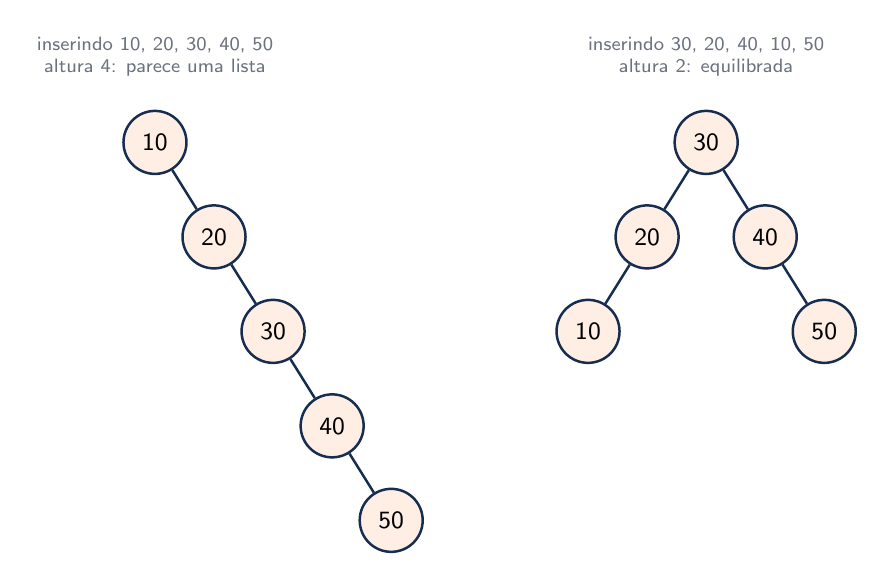
\begin{tikzpicture}[arvore]
  % degenerada: 10, 20, 30, 40, 50
  \node[vertice] (d) at (0,0) {10}
    child[missing] child {node[vertice] {20}
      child[missing] child {node[vertice] {30}
        child[missing] child {node[vertice] {40}
          child[missing] child {node[vertice] {50}}}}};
  \node[legenda, above=3mm of d, align=center] {inserindo 10, 20, 30, 40, 50\\altura 4: parece uma lista};

  % balanceada: 30, 20, 40, 10, 50
  \node[vertice] (b) at (7,0) {30}
    child {node[vertice] {20} child {node[vertice] {10}} child[missing]}
    child {node[vertice] {40} child[missing] child {node[vertice] {50}}};
  \node[legenda, above=3mm of b, align=center] {inserindo 30, 20, 40, 10, 50\\altura 2: equilibrada};
\end{tikzpicture}
\end{document}
